\subsection{Noise and it's Cancellation by LIGO}

Any disturbance in the surrounding could potentially act as noise for LIGO which tends to interfere with the detector and could produce it's own signal instead of a gravitational wave. So changes in environment like vibrations in earth's crust, movement of vehicles, tides, winds, volcanic eruption, mining, etc. Even intensive changes like Temperature. And even the limitations of systems can add it's own noise to the signal. So broadly noise can be classified into:

\begin{itemize}
    \item Seismic Noise
    \item Thermal Noise
    \item Optical Noise
\end{itemize}

\subsubsection{Seismic Noise}

A gravitational wave is measured by monitoring the relative distance between two test mass surfaces. Any force affecting the centre of mass would then result in an ambiguous and faulty measurement. A ground-based interferometer is mechanically coupled to the earth and the masses are prone to seismically driven vibrations. The dominant part of the seismic power spectrum is at low frequencies. A moderately quiet site will have a spectrum of roughly,

\begin{equation}
    x(f) = \frac{1}{f^2} \times 10^{-8}m(Hz)^{3/2}
\end{equation}

where $x(f)$ is Band-width of the noise as a function of frequency($f$).


\subsubsection*{Passive technique of seismic noise reduction} 
    
It utilizes the inertial response of a mass on a spring. Passive isolation takes advantage of the fact that above the resonant frequency, $f_0$, of the mass-spring system, the response of the mass to driving forces decreases by $(\frac{f_0}{f})^2$ . Systems with lower resonant frequencies give higher isolation at a given frequency. These passive systems can also be staged by suspending one isolation system from the isolated stage of a previous system. The total isolation then is the product of each mass-spring system, $(\frac{f_0}{f})^{2n}$, where `$n$' is the number of stages (assuming the same resonant frequency).
    
\subsubsection*{Active technique of seismic noise reduction}
    
Active isolation techniques employ a bootstrapping method. A proof mass is placed on the platform being isolated. The proof mass is more inertial than the platform it sits on. Monitoring the relative displacement, velocity, or acceleration between the platform and the proof mass generates an error signal when the platform has suffered a disturbance to its state. Feedback control systems are used to correct the error signal, locking the position of the platform to the inertial reference of the proof mass. The level of isolation is proportional to the closed-loop gain of the system when the sensor noise is low enough. The limits to the closed-loop gain, the isolation are the sensor’s bandwidth and noise. An advantage to arranging the isolation system in stages is that loop gain in each stage can be more modest, which is sometimes forced by the available bandwidths and mechanical resonances of the structure.\\

LIGO I uses a simple, multi-layer passive isolation system which places a “wall” in the seismic noise spectrum at roughly 40 $Hz$. The proposed LIGO II seismic isolation is largely active \cite{giaime2000active}. A quiet hydraulic system is used externally to the vacuum chambers which house the test masses. This external system has large dynamic range, and is used primarily to take-out long-time scale drifts and disturbances. A two-stage active isolation system inside the test mass chambers is supported by the external system through bellows. The active system isolates an optical table in all six degrees of freedom, from which the test mass is hung as the lower mass of a quadruple pendulum. This design is expected to move the seismic wall to $ \sim 10 Hz$


\begin{figure}[h]
    \centering
    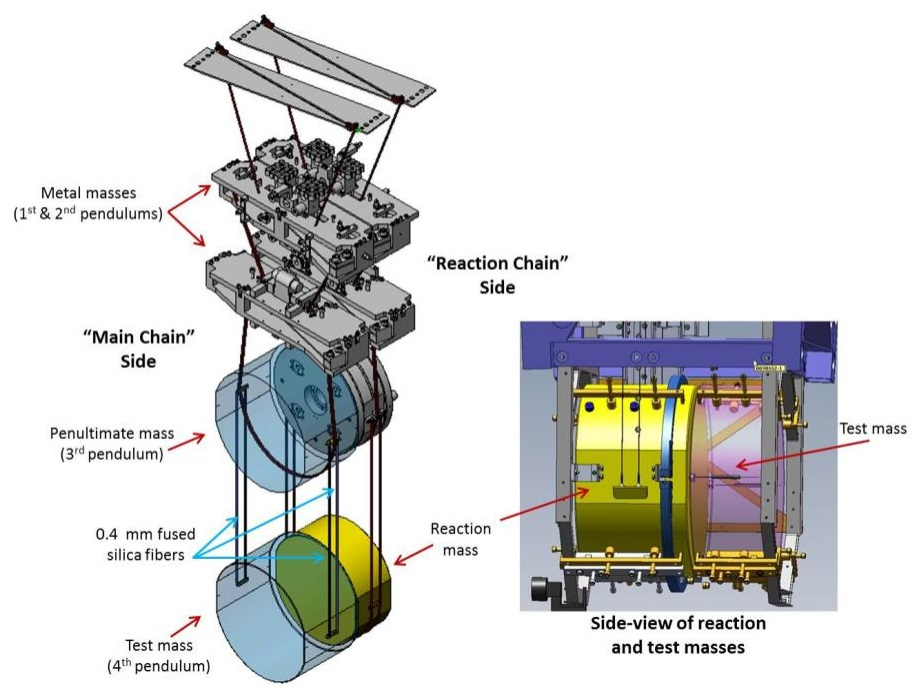
\includegraphics[scale = 1]{images.tex/seismic_isolation.jpg}
    \caption{Mechanism to isolate seismic noise. Source :- \href{https://www.ligo.caltech.edu/page/vibration-isolation}{LIGO.caltech.edu}}
\end{figure}

\subsubsection{Thermal Noise}

Another noise source is due to the fact that the masses are at finite non-zero temperature. Non-zero temperature dictates that the atoms which comprise the masses, as well as the wires which suspend the masses, vibrate, according to entropy. Vibrations of the test mass atoms cause the surfaces of the mirrors to vibrate, which generates a signal. Thermal noise affecting the surface of the test mass directly is called internal thermal noise while the thermal noise from the suspension wires is called pendulum thermal noise. Fibers having low thermal noise and minimum coupling to test mass displacement have been developed. The suspension for LIGO II has been developed using specifically improved fibre and crystalline coating materials like Al-Ga-As. Fused silica ribbons, which are silicate bonded to the test masses are included in this proposal. It is currently predicted that pendulum thermal noise will only contribute to the sensitivity limit in a small region around $10 Hz$.

\subsubsection{Optical noise}

The last of the fundamental noise sources is a limitation of the measurement process itself. The measurement process involves the interaction of light with the test masses, and the subsequent counting of the signal photons by a photo-detector. This has traditionally been thought of in terms of two uncorrelated sources - the Poissonian statistics of the counting of photons, otherwise known as shot noise, and the Poissonian statistics of the force on the test masses from photons, known as radiation pressure noise. \cite{weiss1972electronically} , \cite{saulson1994fundamentals}. Shot and radiation pressure noise are manifestations of the two quadrature of the vacuum. The square-law photo-diode measures the product of the amplitudes of the vacuum and the coherent light from the laser. Increasing the laser power increases the shot noise sensitivity while the radiation pressure noise sensitivity decreases. In LIGO I, 6 watts of light are incident on the interferometer, and radiation pressure noise is negligible. In LIGO II, however, 120 watts of power are planned, making radiation pressure an important factor. The shot noise spectral density is flat, while the radiation pressure amplitude spectral density has a 1/f shape. At a given frequency, the quadrature sum of the shot and radiation pressure noise can be minimized by using the right amount of power. This defines the standard quantum limit. \cite{braginsky1995quantum}

\begin{equation}
    h_{SQL}(f) = \sqrt{\frac{8\hbar}{(2\pi f)^2 mL^2}} 
\end{equation}
where the minimum level of quantum noise is defined as a function of frequency `$h_{SQL}(f)$', `$m$' is  the mass of the test mass, `$L$' is the length of the interferometer arms, `$\hbar$' is the reduced plank's constant. This is actually a locus of the optimum strain spectral density at frequency `$f$' assuming the optimized input power for that frequency,
\begin{equation}
    P_{SQL} = \frac{mL^2(2\pi f)^4}{4\omega_0}
\end{equation}
where $\omega_0$ is the angular frequency of the light. This limit makes the assumption that the shot noise and the radiation pressure noise are uncorrelated. Recent work has discovered that there are correlations in the radiation pressure noise in signal tuned interferometers. \cite{buonanno18optical},\cite{buonanno2001quantum}. Dozens of layers of optical coatings are used, and the test mass is polished to nanometer smoothness. This precision is required to make sure that a near perfect reflective surface is available. Furthermore, laser power and mirror weight are increased to reduce the amount of optical noise present.
